\documentclass[]{book}
\usepackage{lmodern}
\usepackage{amssymb,amsmath}
\usepackage{ifxetex,ifluatex}
\usepackage{fixltx2e} % provides \textsubscript
\ifnum 0\ifxetex 1\fi\ifluatex 1\fi=0 % if pdftex
  \usepackage[T1]{fontenc}
  \usepackage[utf8]{inputenc}
\else % if luatex or xelatex
  \ifxetex
    \usepackage{mathspec}
  \else
    \usepackage{fontspec}
  \fi
  \defaultfontfeatures{Ligatures=TeX,Scale=MatchLowercase}
\fi
% use upquote if available, for straight quotes in verbatim environments
\IfFileExists{upquote.sty}{\usepackage{upquote}}{}
% use microtype if available
\IfFileExists{microtype.sty}{%
\usepackage{microtype}
\UseMicrotypeSet[protrusion]{basicmath} % disable protrusion for tt fonts
}{}
\usepackage{hyperref}
\hypersetup{unicode=true,
            pdftitle={SALVOS DE LA IGLESIA UNIVERSAL DE TODOS LOS TIEMPOS},
            pdfauthor={Ministerios Elim - Los Ángeles},
            pdfborder={0 0 0},
            breaklinks=true}
\urlstyle{same}  % don't use monospace font for urls
\usepackage{natbib}
\bibliographystyle{apalike}
\usepackage{longtable,booktabs}
\usepackage{graphicx,grffile}
\makeatletter
\def\maxwidth{\ifdim\Gin@nat@width>\linewidth\linewidth\else\Gin@nat@width\fi}
\def\maxheight{\ifdim\Gin@nat@height>\textheight\textheight\else\Gin@nat@height\fi}
\makeatother
% Scale images if necessary, so that they will not overflow the page
% margins by default, and it is still possible to overwrite the defaults
% using explicit options in \includegraphics[width, height, ...]{}
\setkeys{Gin}{width=\maxwidth,height=\maxheight,keepaspectratio}
\IfFileExists{parskip.sty}{%
\usepackage{parskip}
}{% else
\setlength{\parindent}{0pt}
\setlength{\parskip}{6pt plus 2pt minus 1pt}
}
\setlength{\emergencystretch}{3em}  % prevent overfull lines
\providecommand{\tightlist}{%
  \setlength{\itemsep}{0pt}\setlength{\parskip}{0pt}}
\setcounter{secnumdepth}{5}
% Redefines (sub)paragraphs to behave more like sections
\ifx\paragraph\undefined\else
\let\oldparagraph\paragraph
\renewcommand{\paragraph}[1]{\oldparagraph{#1}\mbox{}}
\fi
\ifx\subparagraph\undefined\else
\let\oldsubparagraph\subparagraph
\renewcommand{\subparagraph}[1]{\oldsubparagraph{#1}\mbox{}}
\fi

%%% Use protect on footnotes to avoid problems with footnotes in titles
\let\rmarkdownfootnote\footnote%
\def\footnote{\protect\rmarkdownfootnote}

%%% Change title format to be more compact
\usepackage{titling}

% Create subtitle command for use in maketitle
\providecommand{\subtitle}[1]{
  \posttitle{
    \begin{center}\large#1\end{center}
    }
}

\setlength{\droptitle}{-2em}

  \title{SALVOS DE LA IGLESIA UNIVERSAL DE TODOS LOS TIEMPOS}
    \pretitle{\vspace{\droptitle}\centering\huge}
  \posttitle{\par}
    \author{Ministerios Elim - Los Ángeles}
    \preauthor{\centering\large\emph}
  \postauthor{\par}
      \predate{\centering\large\emph}
  \postdate{\par}
    \date{2019-08-28}

\usepackage{booktabs}
\usepackage{amsthm}
\makeatletter
\def\thm@space@setup{%
  \thm@preskip=8pt plus 2pt minus 4pt
  \thm@postskip=\thm@preskip
}
\makeatother

\begin{document}
\maketitle

{
\setcounter{tocdepth}{1}
\tableofcontents
}
\hypertarget{salvos-de-la-iglesia-universal}{%
\chapter{Salvos de la Iglesia Universal}\label{salvos-de-la-iglesia-universal}}

\begin{quote}
\textbf{Col 1:20} Y por medio de Él reconciliar todas las cosas consigo, habiendo hecho la paz por medio de la sangre de su cruz, por medio de Él, repito, ya sean las que están en la tierra o las que están en los cielos.
\end{quote}

Este es un estudio doctrinal sobre la Iglesia en todos los tiempos, desde una perspectiva universa.

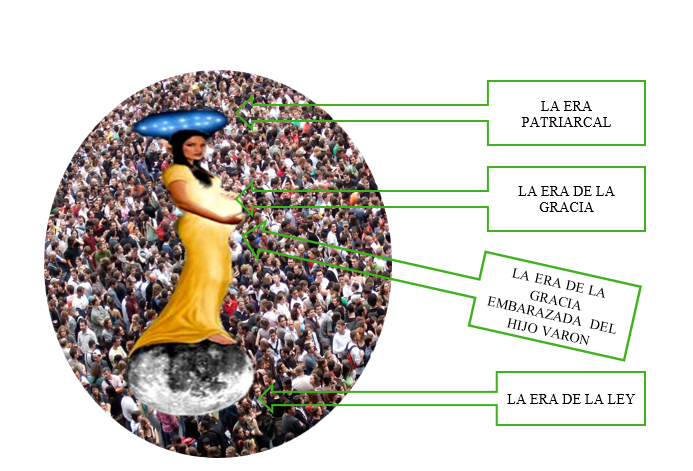
\includegraphics{static/iglesia_universal.png}

\hypertarget{salvos-de-la-iglesia-universal-1}{%
\chapter{Salvos de la Iglesia Universal}\label{salvos-de-la-iglesia-universal-1}}

\begin{quote}
\textbf{Col 1:20} Y por medio de El reconciliar todas las cosas consigo, habiendo hecho la paz por medio de la sangre de su cruz, por medio de Él, repito, ya sean las que están en la tierra o las que están en los cielos.
\end{quote}

Para poder ensenar los últimos tiempos lo primero que debemos debemos hacer es ubicarnos en contexto de los tiempos finales que nos a tocado vivir 1 Cor 10:11 Américas.

Y para entender esto tenemos que estudiar el macrocosmos o macro esquema escatológico, que narra y marca puntualmente la biblia de los hijos de Dios.

Los cuales estamos interesados en nuestro destino final Efe 1:10. y que gracias a su gran misericordia que es mas alta que los cielos salmo 3:11, nos invita a llegar a ese glorioso momento en el cual nos van a galardonar siendo la reina del cielo o esposa de cordero, aunque la base bíblica el pie de imprenta la encontramos en la biblia es por el lado negativo, pero si existe el lado negativo, existe el verdadero. Jeremías 7:18, esto quiere decir que en el cielo hubo, hay o abra una reina del cielo.

Por lo cual empezamos nuestro estudio desde el cosmos lo mas grande, para estudiar quien en son estos hombres y mujeres que serán dignos de este glorioso galardona miento de ser reina de los cielos eternamente, que empieza con nuestro mismo Jesucristo cuando se aparezca a nuestras vidas en su parusías o manifestación secreta apo 22;12. En este recorrido descenderemos de lo macro a lo micro en un viaje a través de las escrituras que es fascinante y glorioso descubriendo y al mismo tiempo revelándonos a nuestro ser trino 1 Tes 5:23 si podemos ser de esta elite que es la novia esposa de hoy en día que en un futuro será la cena del cielo.

Al mismo tiempo veremos en este recorrido las cosas inamovibles para nuestra doctrina (Elim) veremos también lo inamovible para nuestra doctrina Elim, aunque pueda suceder que tengamos diferencia en el micro esquema, pero creemos que nuestro Dios de la gloria no irá revelando a cado uno como ministros de a Dios para que lleguemos a la unidad del conocimiento pleno del Hijo de Dios Efesios 4:13.
Por último, vale la pena perseverar y consagrarnos para ser protagonista de todo esto.

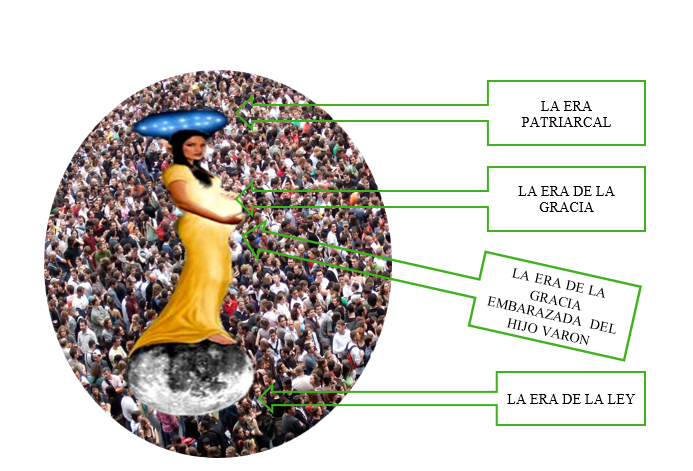
\includegraphics{static/iglesia_universal.png}

\hypertarget{salvos-de-la-iglesia-del-planeta-tierra---desde-adan-hasta-el-trono-blanco.-apoc.-2012}{%
\chapter{Salvos de la Iglesia del planeta Tierra - Desde Adán hasta El Trono Blanco. Apoc. 20:12}\label{salvos-de-la-iglesia-del-planeta-tierra---desde-adan-hasta-el-trono-blanco.-apoc.-2012}}

Continuamos nuestro recorrido escatológico y nos ubicamos en la tierra habitada desde Adam 1Cor 15:45 primera parte. Podríamos decir de Adam el primer hombre caído en la tierra, narrado en la biblia Gen 3:6, aunque dejamos la ventana abierta si hay salvos antes de Adam.

Nos enfocaremos en ese recorrido desde Adam hasta hoy Julio 2019 la biblia nos ensena una sorprendente señal de todos los salvos, me refiero a la señal que le ensenaron al apóstol Juan en Patmos que se encuentra en apoca 12:1-2 en ella nos indica todos los salvos desde que hay memoria de lo escrito a la luz de la biblia en el c0nocimiento histórico de la biblia desde Génesis hasta apocalipsis.

En esta señal de una representación de tres grupos de salvos de toda de las. tres grandes dispensaciones o eras que nos marca la Biblia.

La mujer, vestida de sol, con la luna bajo sus pies, con las estrellas en su cabeza y la mujer misma embarazada representa los salvos de todos los tiempos del planeta tierra desde que hay conocimiento escrito bíblico.

• Grupo numero uno, mujer vestida de sol= a salvos de la era de la gracia
• Segundo grupo, la luna bajo de los pies = salvos de la era de la ley
• Tercer grupo, doce estrellas sobre su cabeza = salvos de la era patriarcal
• Cuarto grupo, el embarazo o niño varón de la mujer vestido de sol, este grupo es de la era de la gracia que se enamoraron de Cristo, Cant .2:5 -Cant 5:8. Y fueron elegidos por la consagración que practicaron al nivel mas alto en la iglesia de Jesucristo hacer parte de niño varón de ese embarazo y que la biblia lo llama primicias. Apo 14:4

Este grupo que seria un subgrupo de los salvos de la gracias o sea la mujer vestida de sol, mueve a todos los salvos de la gracia por los dolores de parto de los cuales se encuentra en la actualidad Ap 12:2.

\hypertarget{los-salvos-de-la-iglesia-de-jesuscristo}{%
\chapter{Los salvos de la Iglesia de JesusCristo}\label{los-salvos-de-la-iglesia-de-jesuscristo}}

\begin{quote}
SON TODOS LOS QUE ESTAN EN LA MUJER VESTIDA DE LUZ APOC. 12:1-2
\end{quote}

\begin{quote}
SON TODOS LOS QUE HAN RECONOCIDO A MI JESUS COMO MI SALVADOR ROM.10:9 CUERPO DE CRISTO 1 COR. 12:27
\end{quote}

En nuestro viaje al microcosmos del esquema escatológico ahora llegamos a la iglesia de Jesucristo que son todos los salvo que han reconocido9 a mi Jesús como su salvador. Rom 10:9-10. Desde que mi Cristo dio su vida, para cumplir lo que decía la ley del padre que el salvador de nuestro ser trino tenia que morir para poder ser salvos nosotros. Heb 9:16-17 por cada uno de los que confesaron con su boca y creyeron en Jesús por fe somos salvos.

1)Estos salvos hoy en día son 2.400 mil millones de cristianos en la tierra que es un 33\% de todos los habitantes de la tierra.

2)De estos cristianos hay 33 mil denominaciones de 238 países alrededor del mundo.

3)Estos cristianos son los que están vivos hoy en día aquí no contamos los que están muertos desde que mi Jesús derramo su sangre y resucito.

4)No tenemos estadísticas de cuantos son los muertos de la iglesia de Jesucristo desde la cruz hasta hoy. Por lo que nos enfocamos en los que estamos vivos y hemos creído y confesamos a Jesucristo como nuestro salvador.


\includegraphics{static/salvos_de_la_iglesia_de_cristo.png}

\hypertarget{la-iglesia-de-jesuscristo-de-la-gracia}{%
\chapter{La Iglesia de Jesuscristo de La Gracia}\label{la-iglesia-de-jesuscristo-de-la-gracia}}

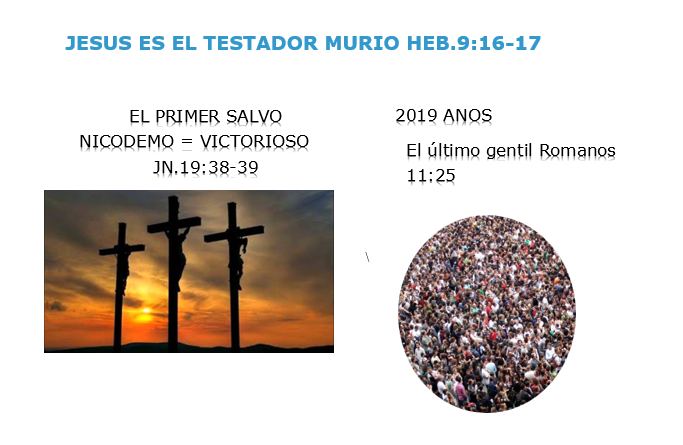
\includegraphics{static/iglesia_de_jesus_cristo_de_la_gracia.png}

\hypertarget{comentarios-finales}{%
\chapter{Comentarios finales}\label{comentarios-finales}}

Dios es tan grande y maravilloso.

\bibliography{book.bib,packages.bib}


\end{document}
